\section{Internal Communication}
\label{design:internalcomm}

We also have to consider internal communication between the bootware core and plugins, and possibly also in between plugins.
Ideally, every plugin will be able to react to events from the bootware.
These event could be triggered by the bootware core or by any plugin, but plugins should be completely independent from each other.
Since a plugin doesn't know about other plugins, it can't listen for events at other plugins directly.
The only known constant to a plugin is the bootware core.
Therefore we need a communication mechanism which allows for loosely coupled communication between the bootware core and the plugins, where plugins can register their interest for certain events with the core and also publish their own events to the core for other plugins to consume.
This essentially describes the publish-subscribe pattern~\autocite{pubsub}.

\subsection{Publish Subscribe Pattern}

The \nom{publish-subscribe pattern}{PubSub} is a messaging pattern that consists of three types of participant: An event bus (or message broker), publishers, and subscribers.
The event bus sits at the center of the communication.
It receives messages from publishers and distributes them to all subscribers that have voiced their interest in messages of a certain type by subscribing at the event bus~\autocite{pubsub}.

Using this pattern in our bootware component, we would create an event bus at the bootware core and plugins, as well as other parts of the core, could subscribe at this event bus and also publish messages through this event bus.

\begin{figure}[!htbp]
	\centering
	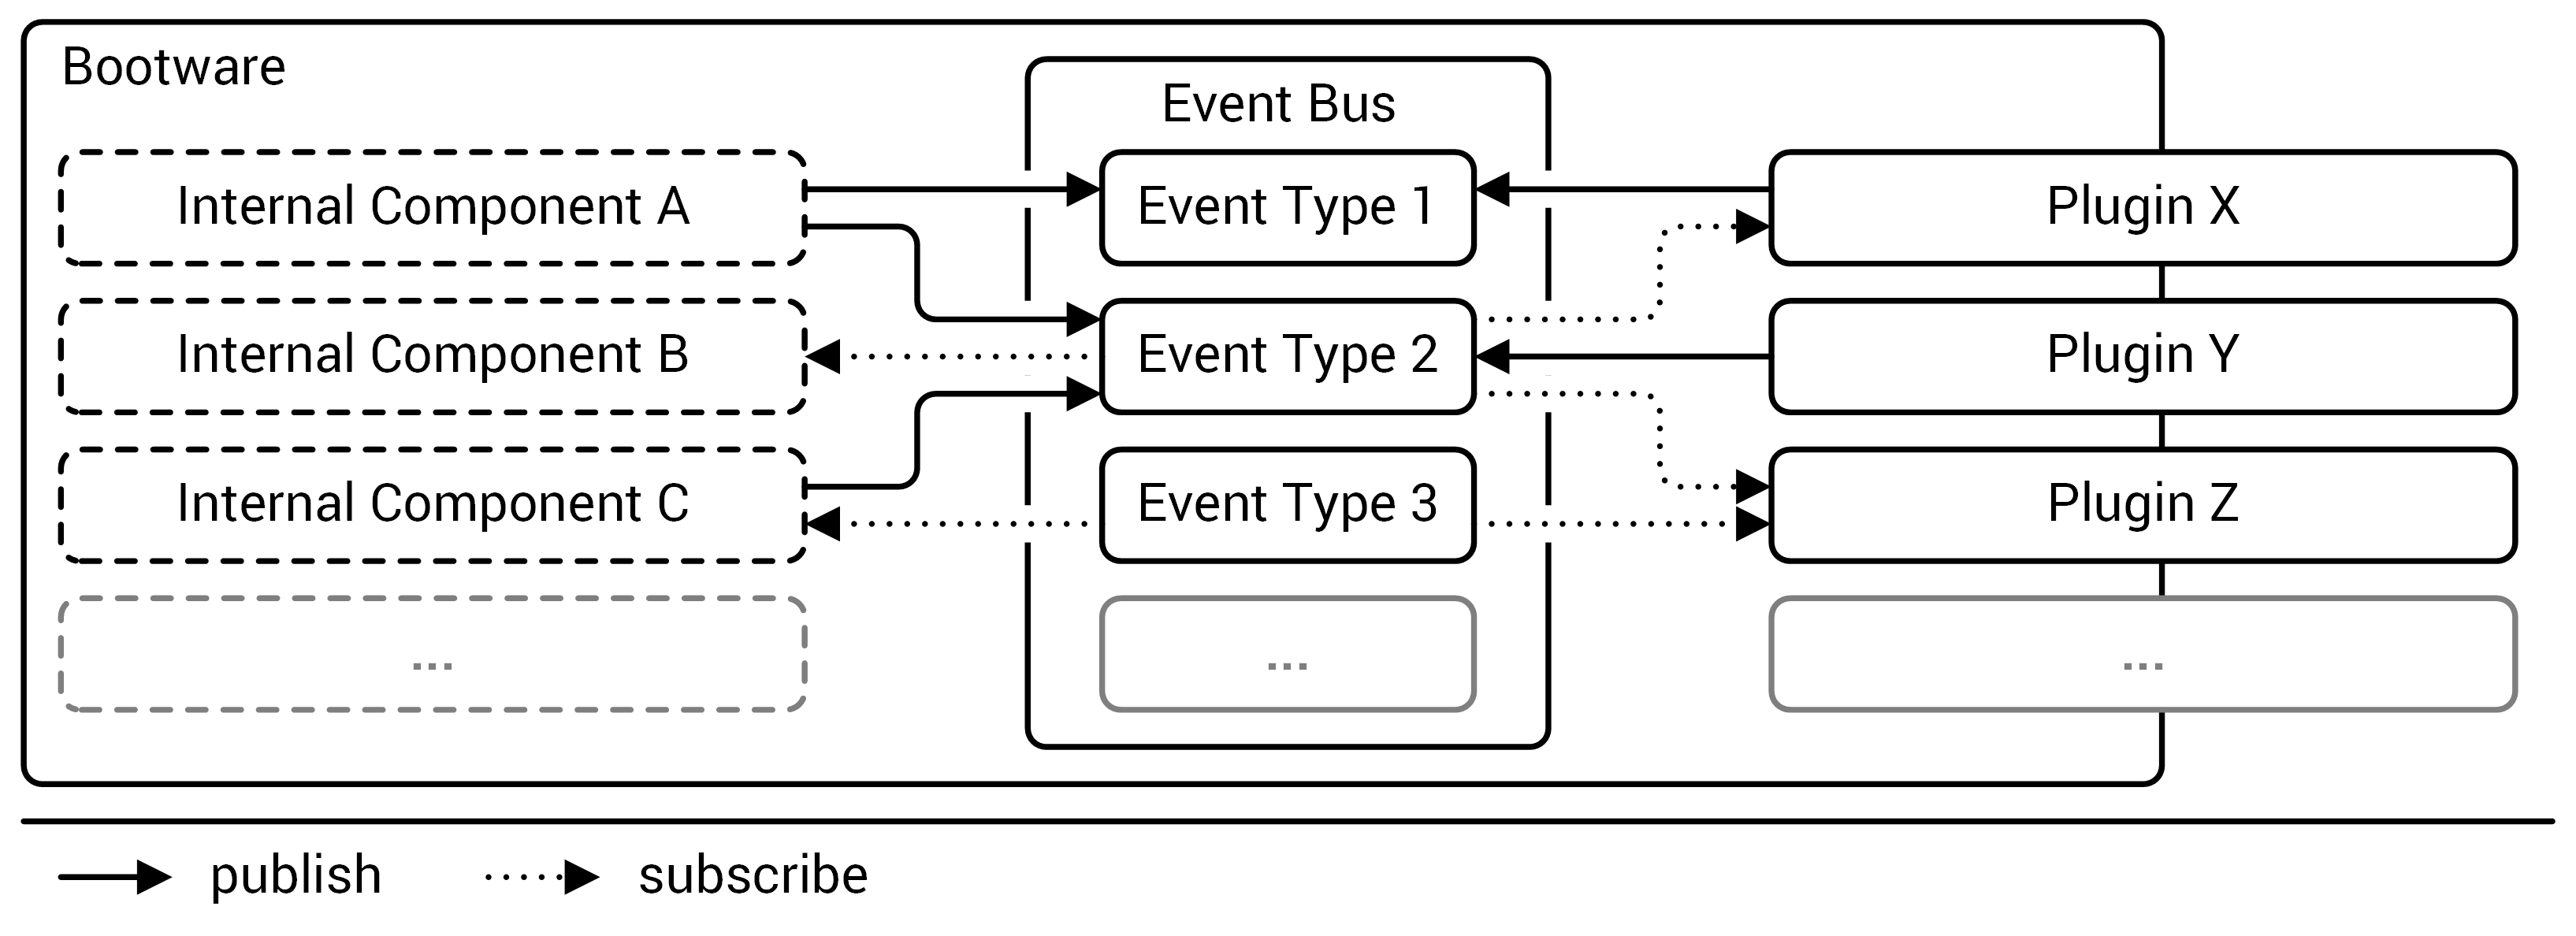
\includegraphics[resolution=600]{design/assets/pubsub}
	\caption{Bootware internal communication with PubSub pattern.}
	\label{image:pubsub}
\end{figure}

\subsection{Event Types}

When using PubSub and events to communicate, its usually a good idea to not only use one type of event, but many different types.
Using different kinds of event allows us to subscribe only to specific events or react differently based on the type of an event.
But what if we want to react to each event type in the same way, for example for logging purposes?
Now, many different event types complicate things more.
This is where event hierarchies become useful.
At the core of an event hierarchy is a single base event.
By extending and refining this base event, other, more specific event types can be created, which again can be used as base type for even more specific events.
This allows us to create a fine grained hierarchy of events and also enables us to subscribe to particular sub sets of this hierarchy.
This makes event handling much easier, since we can now just react to the parent event if we don't need to distinguish between different event types for a particular task.

A second mechanism to differentiate between events is some sort of severity value that each event contains.
Many events will be published in an event system, but not all of them might be of the same importance.
The majority might be of low value while a few events might be very important.
For example, for logging purposes we might not be interested in every event, but only warnings and errors.
By adding a severity attribute to the base event type, all events could be categorized in different severity groups and filtered accordingly if needed.

As we can see, we might benefit from a well thought-out event hierarchy.

\textcolor{red}{
base event
	plugin event
		plugin loading event
		plugin execution event
	state machine event
		transition event
		start event
		stop event
}
